% !TeX TXS-program:compile = txs:///pdflatex/[--shell-escape] 

\documentclass[11pt,a4paper,titlepage,german]{article}

\usepackage[utf8]{inputenc}
\usepackage{authblk}
\usepackage{blindtext}
\usepackage{verbatimbox}
\usepackage{hyperref}
\usepackage[T1]{fontenc}
\usepackage{babel}
\usepackage{graphicx}
\usepackage{color}
\usepackage[dvipsnames]{xcolor}

\definecolor{CGreen}{HTML}{7ac142}
\definecolor{CBlue}{HTML}{5283c1}
\definecolor{CYellow}{HTML}{F9A825}

\graphicspath{ {img/} }

\newcommand*{\email}[1]{%
	\normalsize\href{mailto:#1}{#1}\par
}

\title{\texttt{RunItEasy}\\ \textbf{Benutzerhandbuch}}
\author{
	Peeters, Noah\\ \texttt{noah.peeters@icloud.com}
	\and
	Blechschmidt, Til\\ \texttt{til@blechschmidt.de}
	\and
	Brandt, Merlin\\ \texttt{merlin.brandt@hotmail.de}
	\and
	Clemens, Steffen\\ \texttt{steffen.clemens@hotmail.de}
	\and
	Zager, Max\\ \texttt{max.zager@gmx.de}
	\and
	Schulz, Ron-Niclas\\ \texttt{ronny\_pony@hotmail.de}
	\and
	Tutus, Ayla\\ \texttt{ayla.tts@gmail.com}
	
}
\date{Stand: \today}

\begin{document}
	\maketitle
	
	\begin{abstract}
		Dank der intuitiven Software “RunItEasy” ist es möglich, die Bundesjugendspiele mit geringem Aufwand und hoher Effizienz mit Hilfe modernster Technologien zu bestreiten. Frei von Zetteln mit vorgedruckten Tabellen können dank “RunItEasy” Messergebnisse mit einem Computer, Smartphone oder Tablet digital erfasst und kabellos an die Urkundenschreiber weitergegeben werden. 
	\end{abstract}
	
	\newpage
	
	\tableofcontents
	
	\newpage
	
	\part{Serververwaltung}
		\section{Installation}
			\label{install}
			\addcontentsline{toc}{subsection}{Benötigte Programme}
			Vor Beginn der Installation ist es von größter Notwendigkeit, dass Sie NodeJS installieren. Laden Sie hierfür die Installationsdateien von der \href{https://nodejs.org/en/download/}{\underline{\color{blue}offiziellen Seite}} herunter und führen Sie sie aus. Zusätzlich benötigen sie \textbf{eine laufende Instanz} eines MongoDB Datenbankservers auf dem Gerät. Das Installationspaket finden sie auf \href{https://www.mongodb.com/download-center}{\underline{\color{blue}http://mongodb.com/}}. Laden Sie diese herunter und führen Sie es ebenfalls aus. Anweisungen zum Starten Ihres eigenen Datenbankservers finden sie auf \href{https://docs.mongodb.com/manual/tutorial/install-mongodb-on-windows/#run-mongodb-community-edition}{\underline{\color{blue}dieser Seite}}. Zu Beginn des Prozesses wird ein Archivierungsprogramm benötigt. Für diesen Zweck ist es empfehlenswert \href{http://www.7-zip.org/download.html}{\underline{\color{blue}7-Zip}} zu installieren, da der Vorgang mit diesem zuvor ausgiebig getestet wurde.
			
			\addcontentsline{toc}{subsection}{Download und Installation von RunItEasy}
			Um “RunItEasy” auf Ihrem Server zu installieren, laden Sie sich die aktuelle, universelle Version von \href{https://github.com/TheMegaTB/BJS/releases}{\underline{\color{blue}GitHub}} herunter und entpacken Sie sie mit dem Programm 7-Zip, welches sie zuvor installiert haben. Innerhalb des Archivs befindet sich dieses Dokument, das Wartungshandbuch sowie die entsprechenden Distributionen für verschiedene Betriebssysteme. Öffnen Sie, basierend auf der folgenden Tabelle, den Ordner, welcher ihrem Betriebssystem entspricht. Dabei entspricht x86 einem 32-Bit System und x86-64 einem 64-Bit.

			\begin{center}
				\def\arraystretch{2}
				\begin{tabular}{ l | l | l }
					\multicolumn{1}{c}{\bfseries Betriebssystem} & \multicolumn{1}{c}{\bfseries Architektur} & \multicolumn{1}{c}{\bfseries Verzeichnisname} \\
					\hline
					Windows & x86 & os.windows.x86\_32 \\
					\hline
					macOS & x86-64 & os.osx.x86\_64 \\
					\hline
					Linux & x86 & os.linux.x86\_32 \\
					 & x86-64 & os.linux.x86\_64
				\end{tabular}
			\end{center}
			
			\addcontentsline{toc}{subsection}{Starten des Servers}
			Anschließend führen sie die Datei mit dem Namen “launchBJS.bat” (Windows) bzw. “launchBJS.sh” (Linux, macOS) aus. Es öffnet sich ein Fenster, in welchem Sie die Informationen über den aktuellen Status des Servers ablesen können. Dort finden sie u.a. auch das Administratorpasswort, mit welchem sie Wettkämpfe konfigurieren können. Beziehen Sie sich hierzu auf den Abschnitt “Erstkonfiguration der Bundesjugendspiele”.
			
		\section{Deinstallation}
			Um "RunItEasy” von ihrem Server zu deinstallieren, löschen sie den Ordner, welchen Sie heruntergeladen haben und befolgen sie die Anweisungen zur Deinstallation auf den offiziellen Seiten von NodeJS und MongoDB. Die Hyperlinks zu diesen finden Sie im Bereich “Erstinstallation” dieses Abschnittes.
		
	\newpage
		
	\part{Konzept}
		Dank der intuitiven Software “RunItEasy” ist es möglich, die Bundesjugendspiele mit geringem Aufwand und hoher Effizienz mit Hilfe modernster Technologien zu bestreiten.
		Frei von Zetteln mit vorgedruckten Tabellen können dank “RunItEasy” Messergebnisse mit einem Computer, Smartphone oder Tablet digital erfasst und kabellos an die Urkundenschreiber weitergegeben werden. 
		Dazu muss zunächst der Administrator den Wettkampf konfigurieren, bevor die Bundesjugendspiele beginnen. Für weitere Informationen konsultieren Sie bitte das Kapitel \nameref{concept:initialConfig}.
		Während des Wettkampfes selbst liegen an jeder Station einer Sportart oder bei jeder Gruppe/Klasse ein elektronisches Gerät (Computer, Smartphone oder Tablet) vor, mit dessen Hilfe Messdaten erfasst werden. Nähere Informationen sind in dem Kapitel “Verteilung von RunItEasy” erhältlich.
		Weiterhin müssen die Daten auch zugeordnet werden. Dazu sollte vor Beginn des Wettkampfes jeder Gruppen-/Klassen- und Stationsleiter *in vom Administrator einen Zugangscode bekommen haben. Hierbei ist wichtig festzuhalten, dass nur in der Kooperation von Gruppe und Station Daten erhoben werden können. Weitere Voraussetzungen zur Dateneingabe werden in dem Kapitel “Dateneingabe mit RunItEasy” erläutert. 
		Um die Urkunden erstellen zu können, muss auch den Urkundenschreibern ein elektronisches Gerät vorliegen, auf dem die bereits verarbeiteten Daten zur Eintragung vorliegen. Details dazu sind im Kapitel ”Urkundenerstellung mit RunItEasy” verfügbar.
		
		Der Ablauf der Bundesjugendspiele mit “RunItEasy” sieht daher folgendermaßen aus:
		Der Administrator plant und erstellt einen Wettkampf und gibt persönliche Zugangscodes an die Stations- und Gruppenleiter aus. Gelangt eine Gruppe nun zu einer Station, müssen Gruppen- und Stationsleiter ihre Zugangscodes zusammenbringen, um die Messdaten der Schüler zu erheben. Anschließend werden die Daten von “RunItEasy” verarbeitet und an die Urkundenschreiber digital weitergeleitet.
		
		\section[Konfiguration]{Erstkonfiguration der Bundesjugendspiele}
			\label{concept:initialConfig}
			Damit “RunItEasy” erfolgreich die Bundesjugendspiele begleiten kann, müssen der Software vorab einige Informationen bereitgestellt werden. Dies tut der Administrator in der Erstkonfiguration. 
			Zum einen muss der Administrator festhalten, welche Disziplinen bei den Bundesjugendspielen angeboten werden. Dies ist notwendig, da eventuell aufgrund von Materialbeschränkungen nicht alle möglichen Sportarten durchgeführt werden können oder da Sportarten wie z.B. Sprint elektronisch statt manuell gemessen werden, was zu einer differenzierten Bewertung führt.
			Zum anderen ist es notwendig, alle teilnehmenden Schüler vor Beginn des Wettkampfes einzutragen. Dies muss nicht manuell geschehen, sondern kann auch mit Hilfe von standardisierten CSV-Dateien geschehen.
			
		\section{Externer Zugriff}
			Um mit weiteren Geräten als dem Administrationsgerät auf RunItEasy zuzugreifen, müssen diese Geräte in das gleiche Netzwerk, wie der Administrationsgerät gebracht werden. Dies kann sowohl kabelgebunden als auch kabellos geschehen. Wenn sich die Geräte im Netzwerk befinden, kann RunItEasy über die IP-Adresse des Administrators Computers auf dem Port 8080 erreicht werden (z.B. 198.167.178.21:8080). Diese Adresse ist dem Administrator in der Administrationsübersicht zugänglich und sollte von diesem an die Nutzer verteilt werden. Dies ist nötig, um die Daten mit der Datenbank zu synchronisieren. Nach dem Laden der Website kann RunItEasy auch ohne Verbindung genutzt werden, doch müssen die Daten wieder synchronisiert werden, also mit dem Administrationsgerät verbunden werden.
			
		\section{Dateneingabe}
			Um sicherzustellen, dass die Messergebnisse von Schülern nur dann eingetragen werden können, wenn die Gruppe sich tatsächlich an der Station befindet, ist die Dateneingabe limitiert. So muss vor der Eingabe sowohl die aktuelle Station als auch Gruppe mit den jeweiligen Zugangscodes angemeldet werden. Danach können nur Daten für die Teilnehmer der angemeldeten Gruppe in der aktuell angemeldeten Disziplin erhoben werden. Daraus ist Folgendes ersichtlich:
			Die Gruppen- und Stationsleiter müssen stets ihren Zugangscode zugänglich haben. Es brauchen daher nicht Gruppenleiter und Stationsleiter beide ein Eingabegerät. Es genügt also, wenn jede Station ein Eingabegerät oder wenn jede Gruppe ein Eingabegerät zur Verfügung hat.
			Weiterhin bleibt festzuhalten, dass Messdaten vor dem Auslesen oder Editieren derselben durch Dritte geschützt sind. Das hat zur Folge, dass nach der Abmeldung einer der beiden beteiligten Accounts die eingegeben Daten nicht mehr editierbar sind. Vor der Abmeldung sollten die Eingaben also dringend auf Fehleingaben überprüft werden.
			
		\section{Urkundenerstellung}
			Der letzte Teil der Bundesjugendspiele stellt die Erstellung der Urkunden da. Auch hier erleichtert RunItEasy die Arbeit sehr, da die Messergebnisse nicht noch errechnet werden müssen. Die Software gibt alle notwendigen Daten (Name, Urkundentyp, Gesamtpunktzahl) direkt an, sodass der Prozess deutlich beschleunigt werden kann.
			Ebenso erlaubt RunItEasy die Nutzung mehrer Geräte zum Schreiben der Urkunden, ohne dass einzelne Urkunden mehrfach bearbeitet werden. Um dies zu gewährleisten, muss der Urkundenschreiber nach dem Fertigstellen einer Urkunde selbige als bearbeitet markieren, woraufhin sie anderen Urkundenschreibern nicht mehr angezeigt wird. Näheres zu diesem System finden Sie im Kapitel “Nutzung”.
		
	\newpage
		
	\part{Nutzung}
		\section{Konfiguration}
			\begin{enumerate}
				\item Öffnen sie die Anwendung "RunItEasy", indem sie auf dem zuvor in Abschnitt \ref{install} eingerichteten Server eine Browseranwendung (Chrome, Firefox, Safari) öffnen und \href{http://localhost:8080/}{\underline{\color{blue}localhost:8080}} in die Adresszeile eingeben. Sie sollten daraufhin die nachfolgende Anmeldeseite erreicht haben.\\
				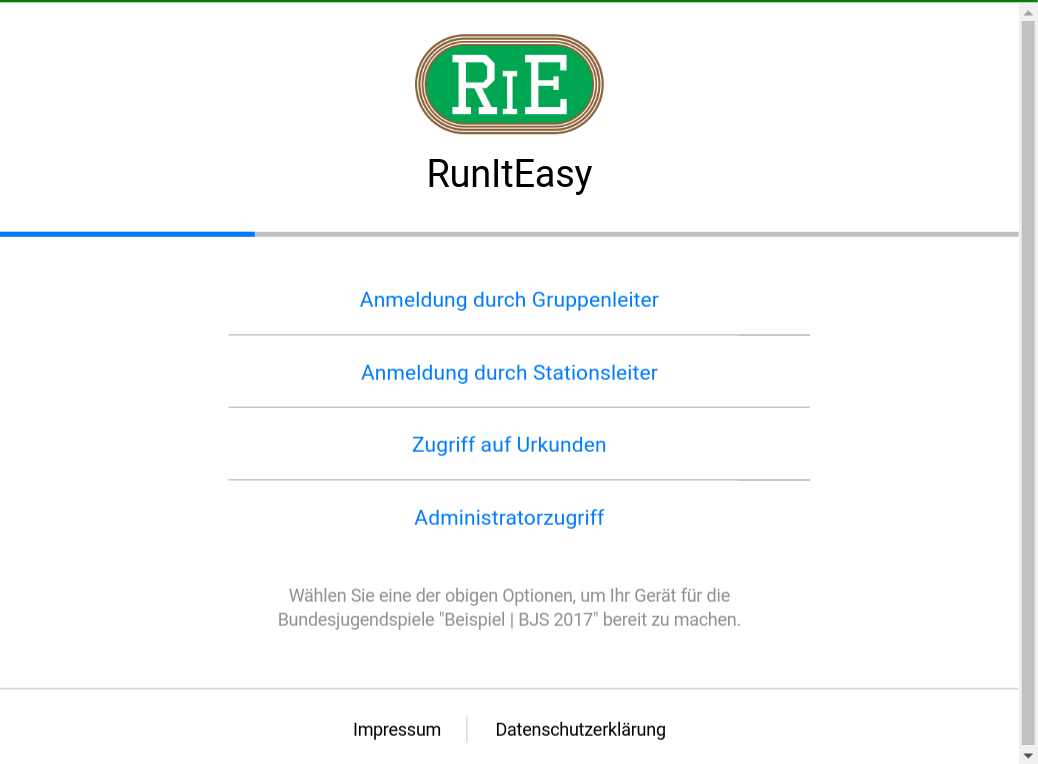
\includegraphics[width=\textwidth]{Login}
				
				\item Um die Konfiguration zu starten, klicken sie auf \texttt{Administratorzugriff} und geben sie das Passwort ein, was ihnen in der Serverkonsole (siehe \nameref{install}) ausgegeben wurde.
				
				\item \addcontentsline{toc}{subsection}{Wettkampfstatus}
					Sie sehen nun eine Übersicht über alle Wettkämpfe, die in dem System sind. Es gibt 3 verschiedene Arten von Wettkämpfen in dieser Ansicht.
					\begin{itemize}
						\item \texttt{Aktiver Wettkampf}. Dieser gleicht dem konfigurierten Wettkampf und ist aktuell aktiv. Er ist mit einer \textbf{\color{CGreen}grünen} Markierung versehen.
						\item \texttt{Konfigurierter Wettkampf}. Ein solcher Wettkampf ist vollständig konfiguriert und kann nicht mehr bearbeitet werden. Er ist mit einer \textbf{\color{CBlue}blauen} Markierung versehen.
						\item \texttt{Unkonfigurierter Wettkampf}. Dies beschreibt einen Wettkampf, dessen Einrichtung noch nicht beendet ist. Bevor diese nicht vollzogen wurde, kann ein solcher nicht aktiviert werden. Er ist mit einer \textbf{\color{CYellow}gelben} Markierung versehen.
					\end{itemize}
				
				\item \addcontentsline{toc}{subsection}{Wettkampf erstellen}
					Indem sie auf den Knopf mit der Aufschrift \texttt{Neuen Wettkampf erstellen} klicken, beginnen einen neuen Wettkampf einzurichten. Zunächst wählen sie die Art des Wettkampfes, den sie anbieten wollen. Anschließend geben sie in das blaue Feld einen sinngemäßen Namen für ihren Wettkampf ein und bestätigen diesen mit einem Klick auf \texttt{Wettkampf erstellen}.
				
				\item \addcontentsline{toc}{subsection}{Wettkampf konfigurieren}
					Sie können einen unkonfigurierten Wettkampf vervollständigen, indem sie diesen in dem rechten Abschnitt anklicken und anschließend \texttt{Bearbeiten} anwählen.
				
					\begin{enumerate}
						\item[Sportarten] Auf dieser Seite wählen sie diejenigen Sportarten, welche sie anbieten möchten beziehungsweise anbieten können. Ist der Schalter grün, so bieten sie diese Sportart an. Sobald die Auswahl ihres Angebotes entspricht, klicken sie auf \texttt{Weiter}
						
						\item[Athleten] Diese Seite dient zur Eingabe der Teilnehmer ihrer Veranstaltung. Die einfachste Methode, dies zu tun ist mittels einer CSV-Datei, welche die benötigten Daten ihrer Teilnehmer beinhaltet (Vorname, Nachname, Geschlecht, Geburtsjahr sowie die Gruppenzugehörigkeit). Klicken sie hierzu auf \texttt{CSV Datei importieren} und wählen sie die Zuordnung der Felder aus. Sie sehen in der rechten Spalte ein Beispieldatensatz. Stimmen die Zuordnungen, so können sie mit dem Import der Daten beginnen, indem sie auf \texttt{Import starten} klicken.\\
						Haben Sie keine CSV-Datei mit den Teilnehmerdaten, müssen Sie diese manuell eingeben. Dazu klicken Sie auf \texttt{Gruppe hinzufügen}. Wählen Sie einen Namen für die Gruppe und bestätigen mit \texttt{OK}. Nun haben Sie mit einem Klick auf \texttt{Athleten hinzufügen} die Möglichkeit, Mitglieder in der Gruppe zu erstellen. Sie können natürlich weitere Gruppen auf die gleiche Weise erstellen und ihnen auch Mitglieder hinzufügen. Darüber hinaus können Sie über das  Suchfeld Mitglieder suchen, um festzustellen, ob sich diese bereits mit den richtigen Daten im System befinden. Wenn Sie fertig sind, klicken Sie auf \texttt{Weiter}.
						
						\item[Zugangscodes] Im letzten Schritt müssen Sie Zugangscodes für die Gruppen, Stationen und Urkundenersteller erzeugen. Standardmäßig wird ein Account für jede Sportart und jede Gruppe, sowie einer zum Erstellen von Urkunden vorkonfiguriert. Da bei der Durchführung der Bundesjugendspiele meistens mehrere Sportarten an einer Station durchgeführt werden (z.B. alle Arten von Sprint), gibt es die Möglichkeit eigene Zugangscodes zu erstellen. Klicken Sie dafür auf \texttt{Eigenen Zugangscode erstellen} und geben Sie anschließend einen Namen ein. Wenn Sie nun auf den Namen des neuen Accounts klicken, können Sie dem Account Rechte geben. Wählen Sie dazu beliebig viele Sportarten aus.
						\\
						Abschließend müssen die eigentlichen Passwörter erstellt werden. Klicken Sie dazu einfach auf \texttt{Passwörter erzeugen}. Sie können die Passwörter über die Schaltflächen in der oberen rechten Ecke  als Textdatei erhalten oder mit 
\includegraphics[height=0.5cm]{DownloadPWD} drucken. Ihr Browser wird Ihnen außerdem die Möglichkeit geben die Passwörter als PDF zu speichern statt zu drucken.
						\\
						\textbf{Hinweis: Diese Passwörter sind aus Sicherheitsgründen nur in dieser Ansicht einsehbar. Sie können später nicht mehr darauf zugreifen. Daher ist es notwendig, dass Sie die Passwörter in diesem Schritt speichern oder anderweitig festhalten. Bei Verlust der Passwörter muss der Wettkampf neu konfiguriert werden.
						}
					\end{enumerate}
					Um den Wettkampf einsatzbereit zu machen klicken sie nun auf \texttt{Konfiguration abschließen}. Beachten sie, dass sie keinerlei Veränderungen mehr vornehmen können, wenn sie diesen Schritt passiert haben, und es nichtmehr möglich ist, die Passwörter einzusehen.
					
				\item \addcontentsline{toc}{subsection}{Wettkampf aktivieren}
					Aktivieren sie nun den neu erstellten Wettkampf, indem sie ihn anklicken und anschließend durch einen Klick auf \texttt{Wettkampf starten} starten. Sollte zuvor ein Wettkampf aktiv gewesen sein, so wird dieser gestoppt.
			\end{enumerate}
		
		\section[Anmeldung]{Anmeldung einer Station oder Gruppe}
			\label{login}
			Geben sie die Adresse, welche sie vom Administrator erhalten haben in ihren Webbrowser (Firefox, Safari, Chrome) ihres Gerätes ein. Sie erhalten eine Oberfläche, die dieser entspricht. Ist dies nicht der Fall, so konsultieren sie bitte den Administrator.\\
			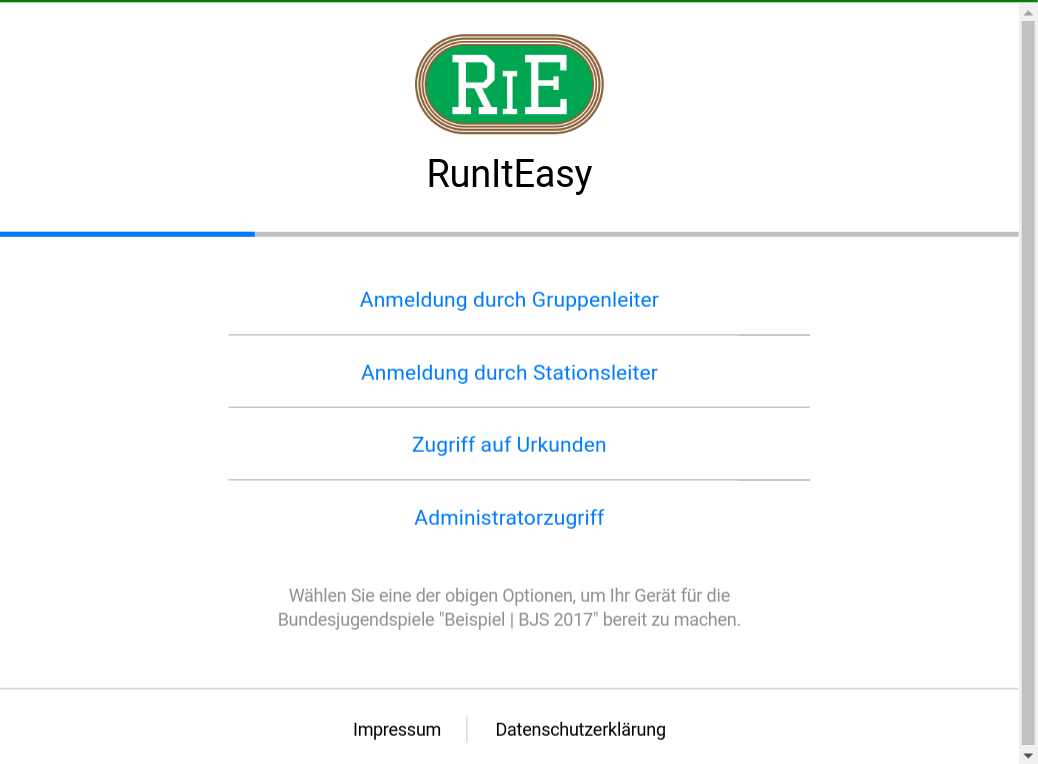
\includegraphics[width=\textwidth]{Login.png}
			Klicken Sie auf “Anmeldung durch Gruppenleiter”, wenn Sie ein Gruppenleiter sind, oder “Anmeldung durch Stationsleiter”, wenn Sie eine Station leiten.  Geben Sie nun das Passwort, welches Sie vom Administrator bekommen haben, in das Feld “Passwort” ein. Sie sollten daraufhin eine der beiden nachfolgenden Seiten erreicht haben.\\
			\addcontentsline{toc}{subsection}{Gruppenlogin}
			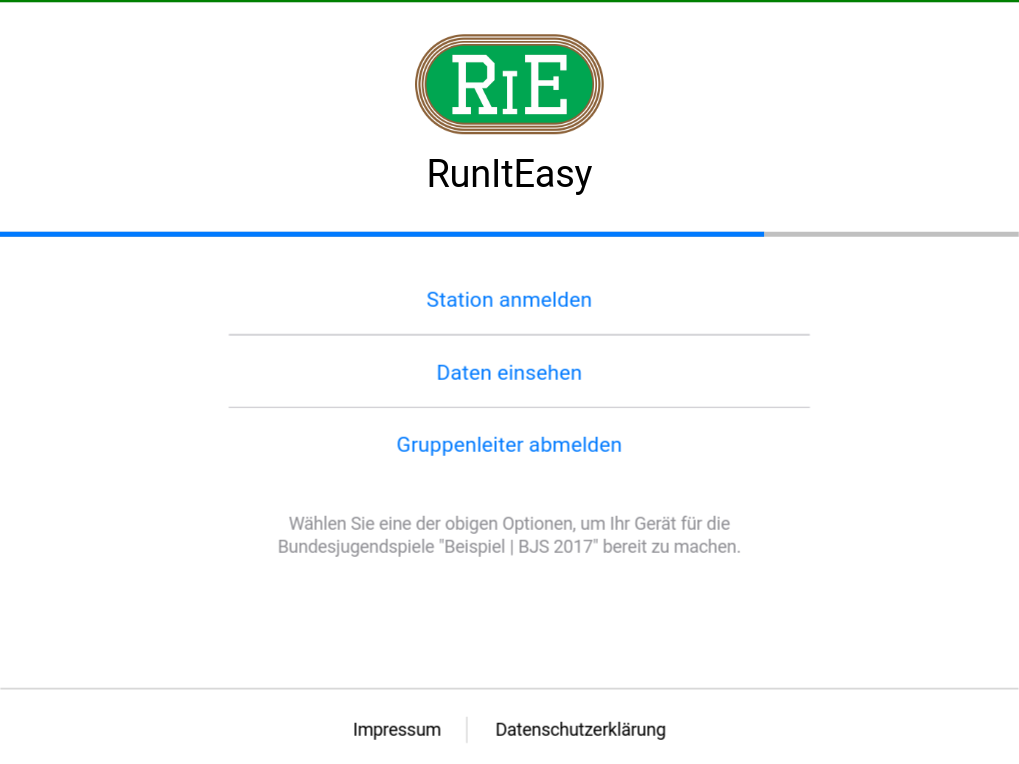
\includegraphics[width=\textwidth]{LoggedIn-Group}
			\addcontentsline{toc}{subsection}{Stationslogin}
			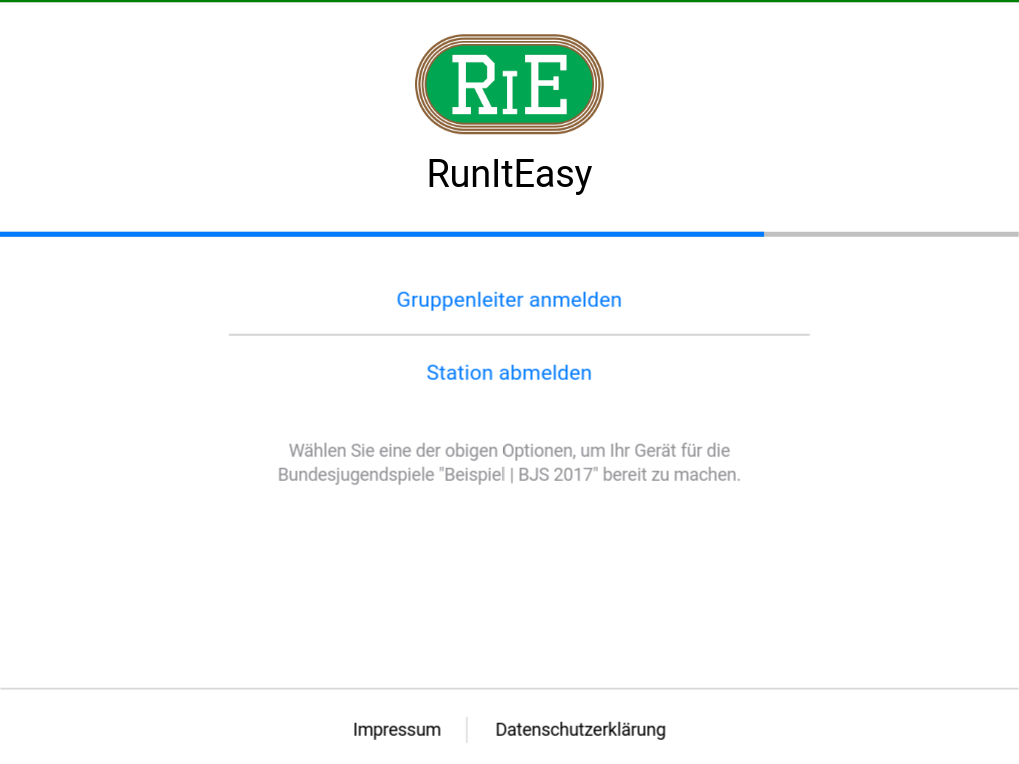
\includegraphics[width=\textwidth]{LoggedIn-Station}
			
		\section[Datenerfassung]{Eingabe von Daten während der Bundesjugendspiele}
			Nachdem Sie sich zuvor als Gruppenleiter (entsprechend Abschnitt \ref{login}) angemeldet haben, bitten Sie den Leiter der Station, an der Sie sich gerade befinden, sich auch an ihrem Gerät anzumelden. Klicken sie dazu auf “Station anmelden”. Falls Sie ein Stationsleiter sind, bitten Sie den Gruppenleiter, sich an ihrem Gerät anzumelden. Klicken sie dazu auf “Gruppenleiter anmelden”.
			Nun kann der Stations- oder Gruppenleiter die Daten, die an dieser Station gemessen wurden, für die Teilnehmer der Gruppe in der nachfolgenden Benutzeroberfläche eingeben.\\
			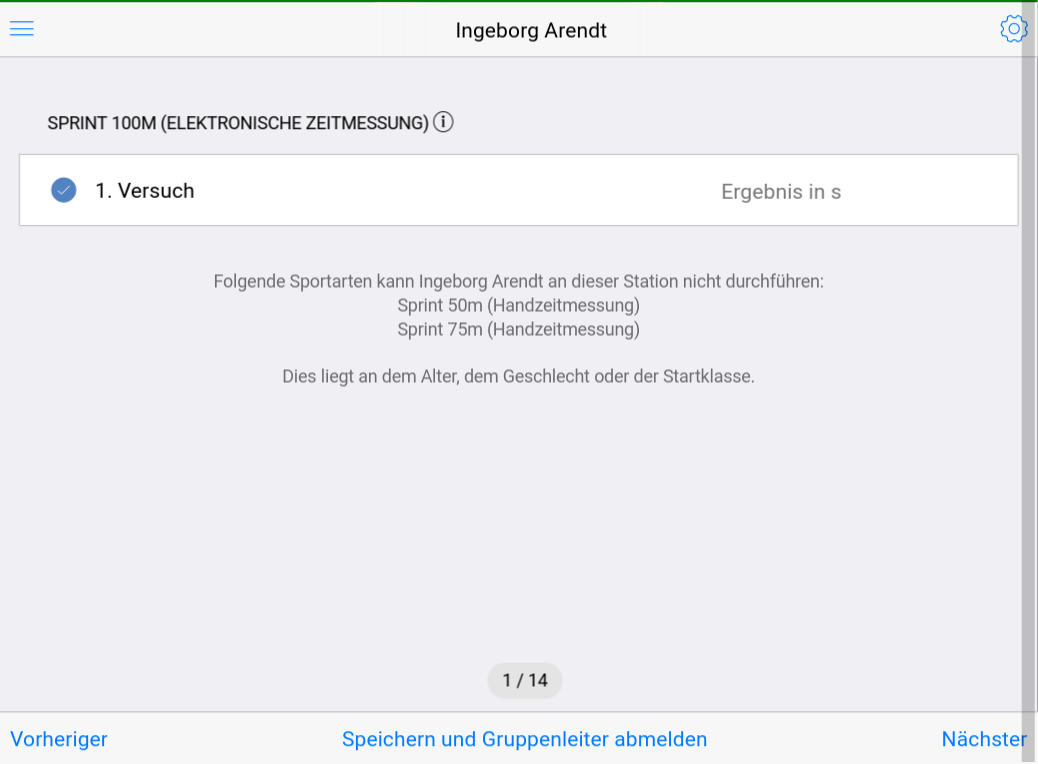
\includegraphics[width=\textwidth]{InputData}
			
		\section{Urkundeneinsicht}
			Die Urkundeneinsicht dient dem Erstellen von Urkunden durch Übertragen der Ergebnisse aus dem Programm auf die Urkunden. Um sich die Ergebnisse anzeigen zu lassen, befolgen Sie folgende Schritte:
			\begin{enumerate}
				\item Rufen Sie die bekanntgegebene Adresse für den Wettkampf in Ihrem Browser (Chrome, Safari, Firefox) auf.
				
				\item Klicken Sie auf \texttt{Zugriff auf Urkunden} und geben Sie das Passwort, welches Sie für die Erstellung der Urkunden erhalten haben, ein und bestätigen Sie mit Enter oder klicken Sie auf \texttt{Anmelden}.
				
				\item Sofern bereits genügend Messdaten für die Athleten eingetragen wurden, sehen Sie nun eine Übersicht der zu erstellenden Urkunden. Ist dies nicht der Fall, so müssen sie warten, bis ausreichend Daten an den Server übertragen wurden.
				
				\item Um einen einfachen und übersichtlichen Arbeitsablauf zu gewährleisten, legen Sie sich zunächst benötigte Urkundenvordrucke bereit.
				
				\item Wählen Sie einen Athleten, in der Regel immer den obersten, aus der Liste aus. Lesen Sie, welcher Urkundentyp erstellt werden muss und nehmen Sie sich den entsprechenden Vordruck.
				
				\item Tragen Sie den Namen und die Gesamtpunktzahl in die dafür vorgesehenen Felder der Urkunde ein. Achten Sie darauf, dass sie das Urkundenpapier dem Urkundentypen entsprechend wählen.
				
				\item Um die Übersicht zu behalten und Urkundenduplikate zu vermeiden, klicken Sie nach jeder fertiggestellten Urkunde auf \texttt{Als erstellt markieren}.
				
				\item Sollten Sie einmal etwas zu früh als erstellt markiert haben, haben Sie die Möglichkeit, als erstellt markierte Urkundeninformationen anzuzeigen. Klicken Sie auf 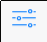
\includegraphics[height=0.5cm]{Settings} oben rechts im Fenster. Anschließend klicken Sie auf 
\includegraphics[height=0.75cm]{CertificateSettings} und aktivieren Sie den Schalter hinter \texttt{Fertig}. Fertiggestellte Urkunden werden nun mit der grünen Markierung am Ende der Liste angezeigt.
				
			\end{enumerate}
		
\end{document}